\chapter{Implementación a nivel de microarquitectura}

En el capítulo anterior se analizaron diferentes tipos de arquitecturas existentes para la implementación de un procesador de descomposición QR. Se describieron sus características a nivel conceptual y se detallaron las definiciones de la arquitectura elegida para realizar la implementación.

En este capítulo se describen las herramientas que fueron utilizadas y se explica en detalle, a nivel de microarquitectura, la forma en la cual fue implementado cada módulo del procesador desarrollado, y la forma en la cual los módulos fueron interconectados para conformar al mismo. Adicionalmente, se describen aquellos desarrollos que fueron el resultado de la presente tesis, utilizados para resolver diferentes necesidades encontradas, los cuales representan un contenido intelectual propio.

La metodología utilizada para el desarrollo del procesador consistió en analizar las necesidades de la arquitectura elegida, y los diferentes componentes requeridos. Se procedió a la definición de dicha arquitectura a través de un diagrama en bloques y se desarrolló cada uno de los módulos por separado, gradualmente. Una vez desarrollado un módulo, se procedió a simular su comportamiento aislado a través de un \textit{testbench} que lograra contemplar el mayor conjunto de los posibles vectores de entrada. Una vez finalizada la simulación individual de los distintos componentes, se procedió a realizar una simulación conjunta de algunos de ellos.

El detalle del código fuente Verilog puede encontrarse en el \autoref{cap:apA}.

\section{Diagrama en bloques}

A continuación se expone un diagrama en bloques a grandes rasgos del hardware desarrollado:

\begin{figure}[!h]
 	\begin{center}
 		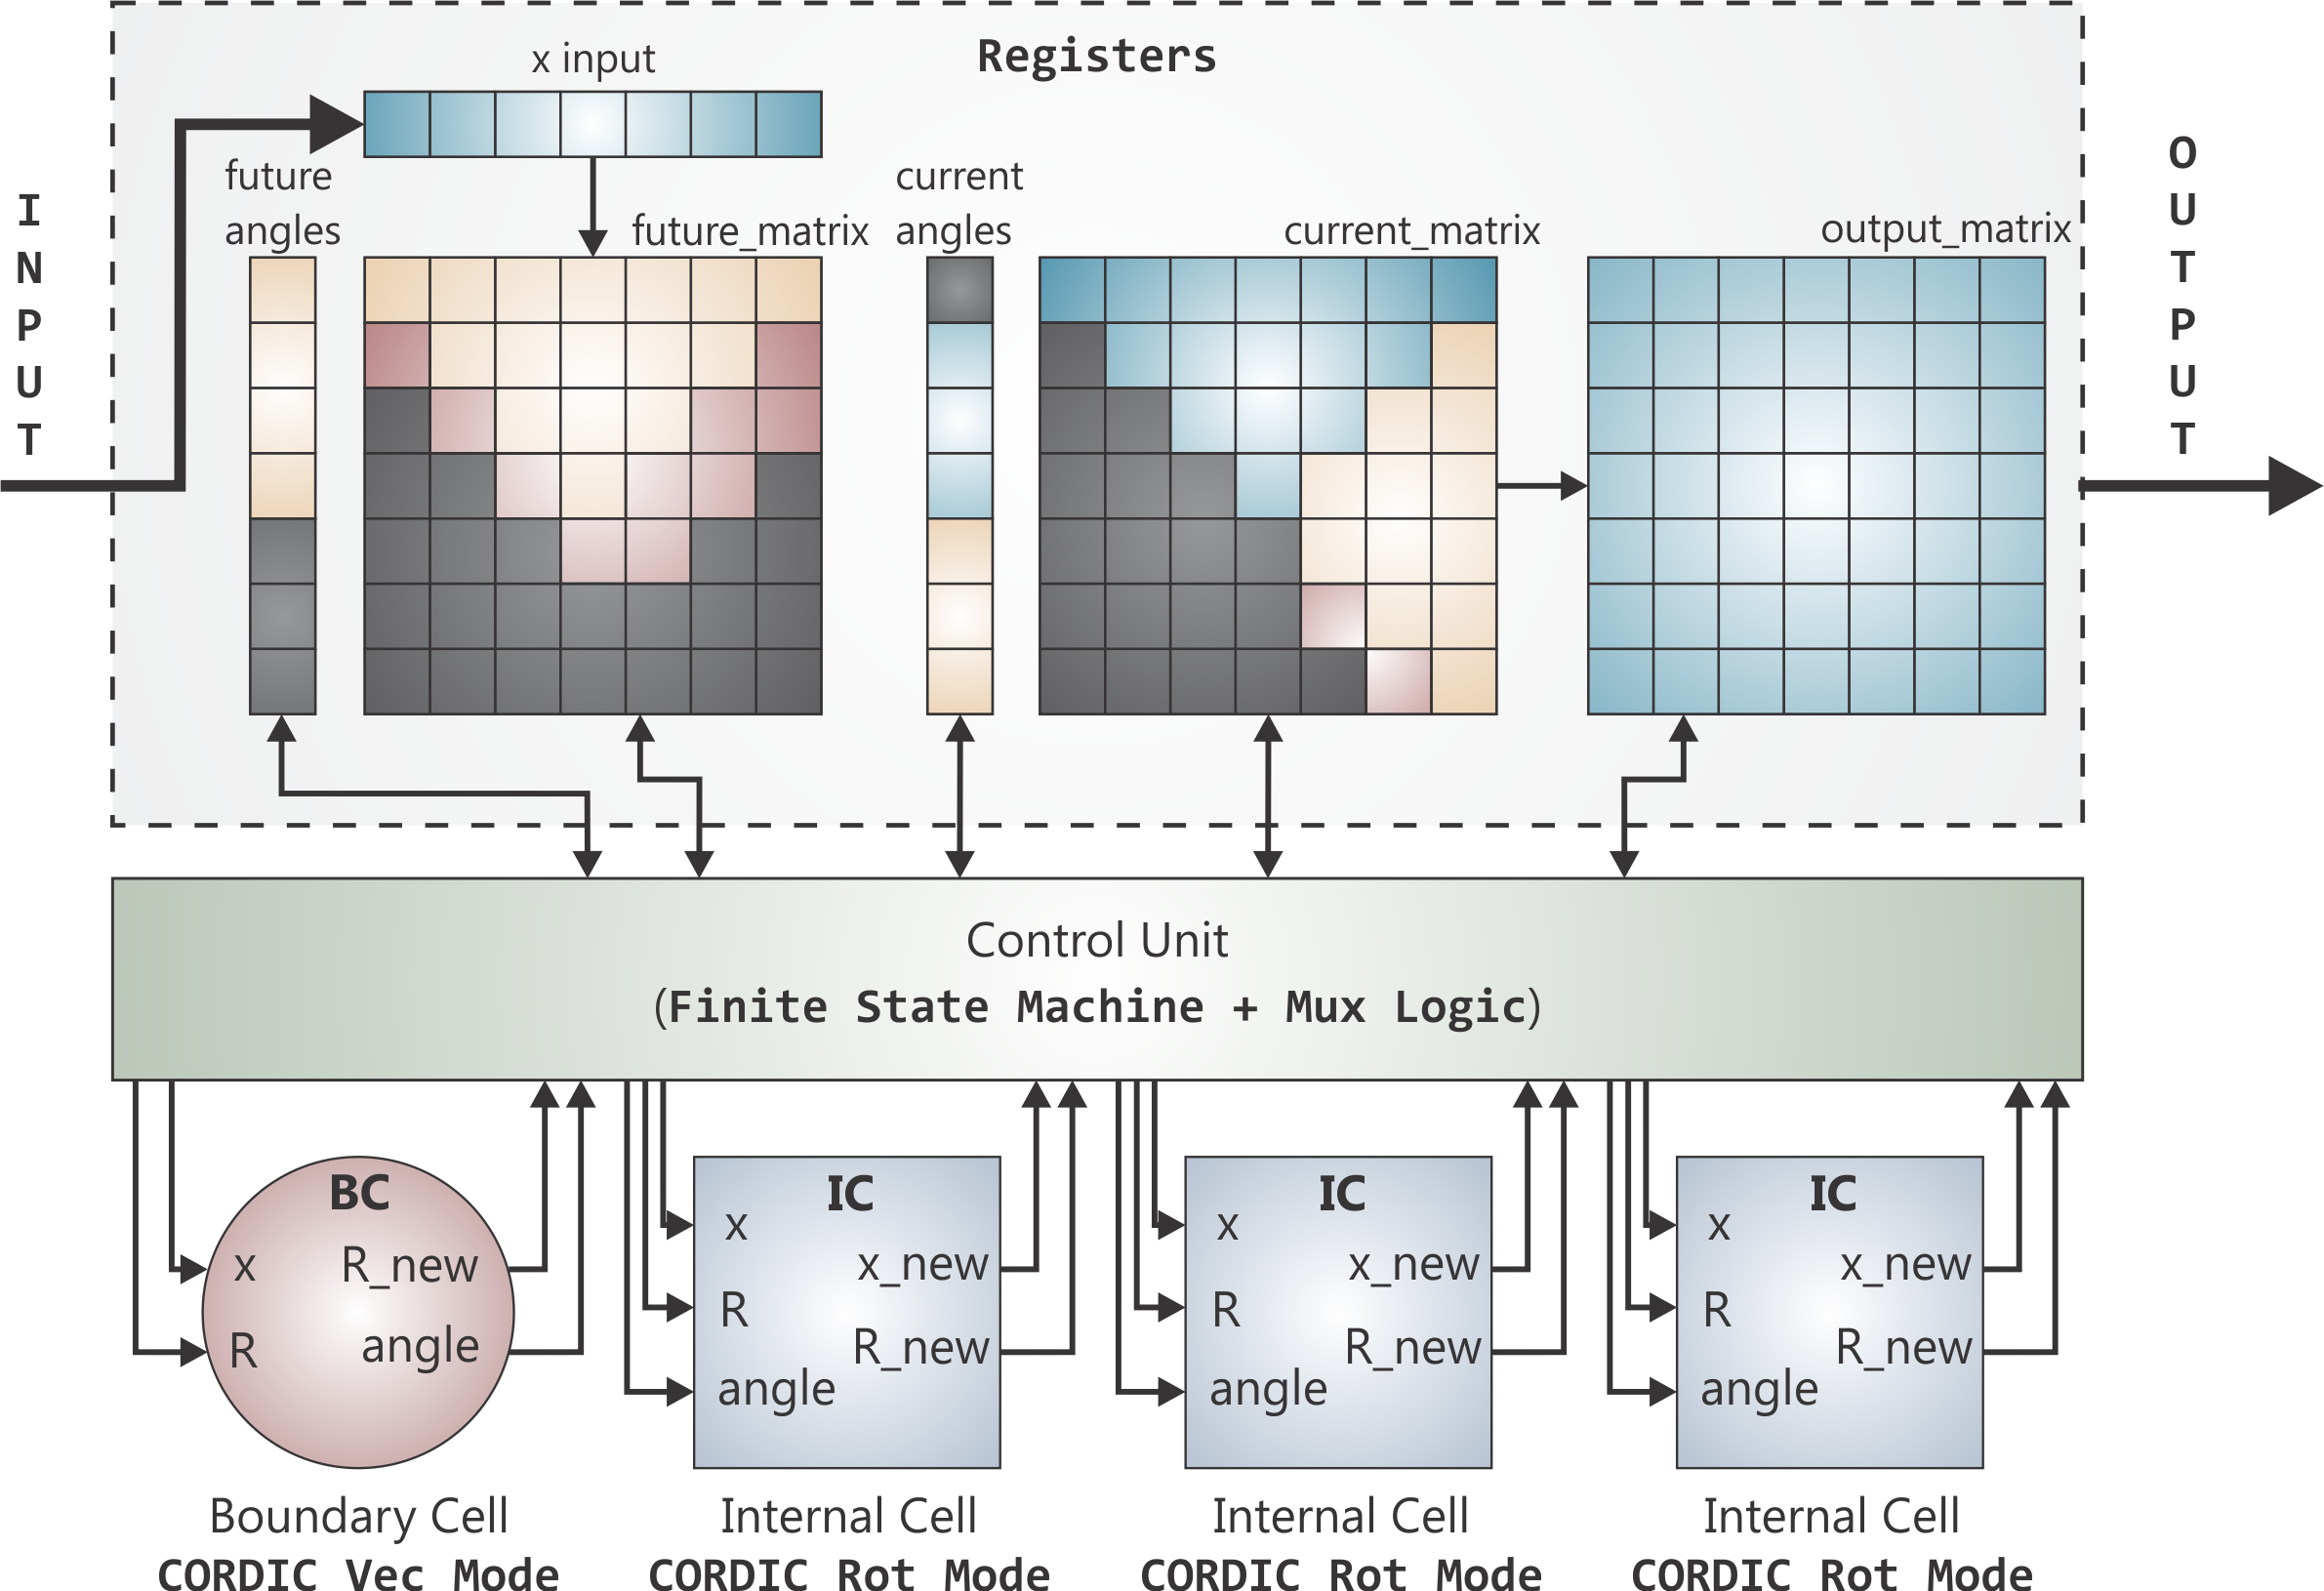
\includegraphics[width=\textwidth]{./figures/C04-block_diagram}
 		\caption{Diagrama en Bloques del Hardware Desarrollado}
		\label{block_diagram}
 	\end{center}
\end{figure}

En el diagrama se pueden observar las unidades desarrolladas para implementar la arquitectura elegida. Las mismas pueden dividirse en 3 grupos:

\begin{itemize}
	\item[•] La unidad de registros contiene el hardware requerido para almacenar los valores de entrada y salida de los procesadores, registrando cada uno de los cálculos realizados. Los datos se encuentran organizados en formato matricial. La unidad fue cuidadosamente desarrollada para adaptarse al comportamiento multiprocesamiento de la arquitectura, y para realizar operaciones de desplazamiento requeridas durante el procesamiento del algoritmo.

	\item[•] La unidad de control es el bloque de hardware que implementa la lógica necesaria para llevar a cabo los pasos del algoritmo según el mapeo de Walke, teniendo en cuenta el vector y las líneas de planificación. Esto se logra a partir del uso de una máquina de estados finita y multiplexores, para direccionar adecuadamente, según el estado actual, las entradas y salidas del hardware.
	
	\item[•] Los procesadores de \textit{boundary cell} e \textit{internal cell} son implementados utilizando núcleos CORDIC. En el caso de las operaciones BC, se utiliza CORDIC en \textit{vectoring mode}, y en el caso de las operaciones IC, el modo utilizado es \textit{rotation mode}. La \textit{boundary cell} es la unidad que toma como entrada los valores de $R$ y $x$ y realiza la rotación de los mismos para obtener el módulo del vector, el cual representa el nuevo valor de $R$, y el ángulo del mismo, el cual es utilizado para enviarlo como entrada a las \textit{internal cells} de la misma fila. Por otro lado, las \textit{internal cells} toman como entrada los valores de $R$, $x$, y el ángulo calculado por las \textit{internal cells}, para dar como resultado el nuevo valor de $R$, y el valor de $x$ para enviar como entrada a la \textit{internal cell} de la siguiente fila.
\end{itemize}

La descripción individual de cada uno de los componentes, empezando desde los módulos más básicos y continuando hasta evolucionar en el \textit{top level}, se encuentra en las siguientes secciones.

\section{Parámetros comunes a los distintos módulos}

\begin{itemize}
	\item[•] \verb;WORD_WIDTH;: Es el parámetro utilizado para definir el ancho de palabra de los datos que representan cada componente de la matriz. El valor por defecto es 16 \textit{bits} y puede soportar hasta 64. El número de iteraciones depende directamente de este valor, por lo cual al aumentar la precisión, aumenta el tiempo de procesamiento requerido.
	\item[•] \verb;ROWS;: Es el parámetro con el cual se define la cantidad de filas de la matriz. Actualmente, la implementación sólo admite que este valor sea 7.
	\item[•] \verb;COLUMNS;: Es el parámetro con el cual se define la cantidad de columnas de la matriz. Actualmente, la implementación sólo admite que este valor sea 7.
\end{itemize}

\section{Pre-procesamiento de entradas para el módulo CORDIC}

El código \textbf{preprocessor.v} describe el hardware desarrollado para hacer el pre-procesamiento de las entradas $x$;$y$;$z$ requerido, antes de enviarlas al procesador CORDIC. Es la primera etapa del módulo de rotación ``\textit{rotator}''. Según fue descripto en la sección \ref{subsec:El_algoritmo_CORDIC}, el procesador CORDIC sólo puede manejar rotaciones entre $-\pi/2$ y $\pi/2$ en cualquiera de sus dos modos de operación. Para aquellos casos en los cuales es necesario hacer rotaciones con ángulos mayores a $\pi/2$ en módulo, es requerido aplicar una rotación inicial de $\pi$.

En el modo rotación, esta transformación se logra negando ambas entradas, $x$ e $y$, y enviándolas al procesador CORDIC. Dicha transformación logra la rotación inicial de $\pi$ deseada, siendo la rotación restante manejada por el procesador CORDIC.  El resultado correcto es extraído directamente desde las salidas del mismo.

En el modo vector, es necesario abordar la transformación desde dos bloques distintos.
En primer lugar, se detecta si el vector de entrada posee un ángulo mayor a $\pi/2$ en módulo observando el signo de la componente $x$. Un ejemplo de dicho caso podría ser el vector $(-1000;1000)$. Estos casos se identifican cuando el signo de $x$ es negativo. En dicho caso, se aplica la misma transformación sobre $x$ e $y$ que se utilizó en el modo rotación, negando las componentes y enviándolas al modulo CORDIC.
En segundo lugar, se debe tomar el ángulo de salida de CORDIC $z_o$, y restarle $\pi$. Esta operación, es manejada por el módulo superior \textbf{rotator.v}.

Para realizar la implementación, se utiliza un \textit{bit} de decisión, el cual según el modo de CORDIC elegido, define qué parámetro será utilizado para determinar si es necesario modificar las entradas:

\begin{lstlisting}[style=C]
vec_rot_n ? d_i <= x_in[WORD_WIDTH-1] : ^z_in[WORD_WIDTH:WORD_WIDTH-1];
\end{lstlisting}

Luego, con el bit de decisión se controlan las entradas x e y y z siguiendo la siguiente lógica:

\begin{lstlisting}[style=C]
Si d_i se encuentra en estado alto entonces
	/* Angulo fuera del dominio valido de CORDIC */
	Asignar x de CORDIC con -x_i y extender 1 bit el signo
	Asignar y de CORDIC con -y_i y extender 1 bit el signo
	Si el modo es rotacion:
		Asignar z de CORDIC con z_i - pi
	sino
		Asignar z de CORDIC con z_i
sino
	/* Angulo dentro del dominio valido de CORDIC */
	Asignar x de CORDIC con x_i y extender 1 bit el signo
	Asignar y de CORDIC con x_i y extender 1 bit el signo
	asignar z de CORDIC con z_i
\end{lstlisting}

Al observar el pseudocódigo es posible identificar que se extienden en un \textit{bit} las entradas del sistema. El motivo de dicha extensión se basa en que, debido a la ganancia de CORDIC, pueden darse casos de overflow para ciertas entradas, y así llegar a resultados erróneos. Para evitarlo, la solución elegida consistió en:

\begin{enumerate}
	\item Extender las entradas en un \textit{bit} en la etapa de pre-procesamiento.
	\item Realizar el cálculo de CORDIC.
	\item Atenuar la ganancia de CORDIC en el módulo de post multiplicación.
	\item Eliminar el \textit{bit} de signo.
\end{enumerate}

De esta forma se adecúa el tamaño de las entradas del procesador CORDIC, evitando la posibilidad de llegar a una condición de overflow.

\section{CORDIC iterativo}

El código \textbf{iterative\_cordic.v} describe el hardware desarrollado para implementar el algoritmo de CORDIC según se encuentra descripto en el \autoref{cap:apC} en su versión iterativa. Lo que se requiere es lograr un hardware que replique las ecuaciones planteadas en \ref{ec3}. La composición del hardware se encuentra diagramada en la figura \ref{fig:cordic_hardware} y se logra como sigue:

\begin{itemize}
\item[•] Por un lado, se tiene un contador que registra el número de iteración dentro del algoritmo. La cantidad de cuentas de dicho contador depende directamente del ancho de palabra utilizado.
\item[•] Se utiliza un \textit{bit} de decisión \verb;di;, el cual trabaja utilizando el signo de $z$ o de $y$ según el modo sea rotación o vectorización.
\item[•] Cuando el hardware se encuentra en el estado \verb;IDLE;, las entradas $x$, $y$, $z$, ingresan en los registros de acumulación. Al salir del estado \verb;IDLE;, el acumulador es actualizado con el contenido de la salida del circuito en cada iteración. Está decisión es implementada por un multiplexor para cada componente $x$, $y$, $z$.
\item[•] $x$ e $y$, son direccionadas a registros de desplazamiento que operan según el número de iteración ( número de \textit{bits} desplazados = número de iteración).
\item[•] Se agregan dos circuitos \textit{add/substract} para implementar las dos ecuaciones de CORDIC. La elección de suma o resta es regida por el \textit{bit} de decisión. Los términos para cada uno son ($x$;$y$ desplazado) por un lado, e ($y$;$x$ desplazado) por el otro.
\item[•] Los valores de arcotangentes elementales son almacenados en una ROM. El acceso a la misma es controlado por el contador de iteraciones del algoritmo. La representación binaria se logra al multiplicar los valores absolutos por una constante para normalizarlos. Se utilizó una constante que normaliza los valores de la tabla para una representación en 64 \textit{bits}, el cual es el máximo valor aceptado por el hardware. En caso de que se utilicen longitudes de palabra menores, se hace un desplazamiento de dichas constantes a derecha (dividir por $2^n$) una cantidad $n = 64 - \text{longitud de palabra}$.

\begin{table}[hp!]
    \begin{center}
    	\footnotesize
        \begin{tabular}{|c|c|c|}
        \hline  
        \textbf{Iteración} & \textbf{Valor de Arcotangente} & \textbf{Representación Decimal de 64 bits} \\
        \hline
			1   &   0,78539816339744800000000   &   4611686018427387904   \\ \hline
			2   &   0,46364760900080600000000   &   2722437224269746380   \\ \hline
			3   &   0,24497866312686400000000   &   1438461061161762076   \\ \hline
			4   &   0,12435499454676100000000   &   0730185295051043895   \\ \hline
			5   &   0,06241880999595740000000   &   0366509582986589657   \\ \hline
			6   &   0,03123983343026830000000   &   0183433460584072433   \\ \hline
			7   &   0,01562372862047680000000   &   0091739112965426259   \\ \hline
			8   &   0,00781234106010111000000   &   0045872355853501789   \\ \hline
			9   &   0,00390623013196697000000   &   0022936527896151662   \\ \hline
			10  &   0,00195312251647882000000   &   0011468307695752815   \\ \hline
			11  &   0,00097656218955931900000   &   0005734159316382967   \\ \hline
			12  &   0,00048828121119489800000   &   0002867080341756270   \\ \hline
			13  &   0,00024414062014936200000   &   0001433540256323779   \\ \hline
			14  &   0,00012207031189367000000   &   0000716770138842597   \\ \hline
			15  &   0,00006103515617420880000   &   0000358385070756387   \\ \hline
			16  &   0,00003051757811552610000   &   0000179192535545079   \\ \hline
			17  &   0,00001525878906131580000   &   0000089596267793400   \\ \hline
			18  &   0,00000762939453110197000   &   0000044798133899308   \\ \hline
			19  &   0,00000381469726560650000   &   0000022399066949980   \\ \hline
			20  &   0,00000190734863281019000   &   0000011199533475031   \\ \hline
			21  &   0,00000095367431640596100   &   0000005599766737520   \\ \hline
			22  &   0,00000047683715820308900   &   0000002799883368761   \\ \hline
			23  &   0,00000023841857910155800   &   0000001399941684380   \\ \hline
			24  &   0,00000011920928955078100   &   0000000699970842190   \\ \hline
			25  &   0,00000005960464477539060   &   0000000349985421095   \\ \hline
			26  &   0,00000002980232238769530   &   0000000174992710547   \\ \hline
			27  &   0,00000001490116119384770   &   0000000087496355274   \\ \hline
			28  &   0,00000000745058059692383   &   0000000043748177637   \\ \hline
			29  &   0,00000000372529029846191   &   0000000021874088818   \\ \hline
			30  &   0,00000000186264514923096   &   0000000010937044409   \\ \hline
			31  &   0,00000000093132257461548   &   0000000005468522204   \\ \hline
			32  &   0,00000000046566128730774   &   0000000002734261102   \\ \hline
        \end{tabular}
        \normalsize
        \caption{Tabla de Arcotangentes}
    \end{center}
\end{table}

\newpage

\item[•] La salida de z se implementa independientemente en forma similar a la de $x$ e $y$, sumando o restando ángulos según el \textit{bit} de decisión, pero tomando como segundo término de la suma/resta el valor de la ROM de arcotangentes, según el valor para la iteración correspondiente.
\end{itemize}

El diagrama del circuito de CORDIC implementado es el siguiente:

\begin{figure}[!h]
 	\begin{center}
 		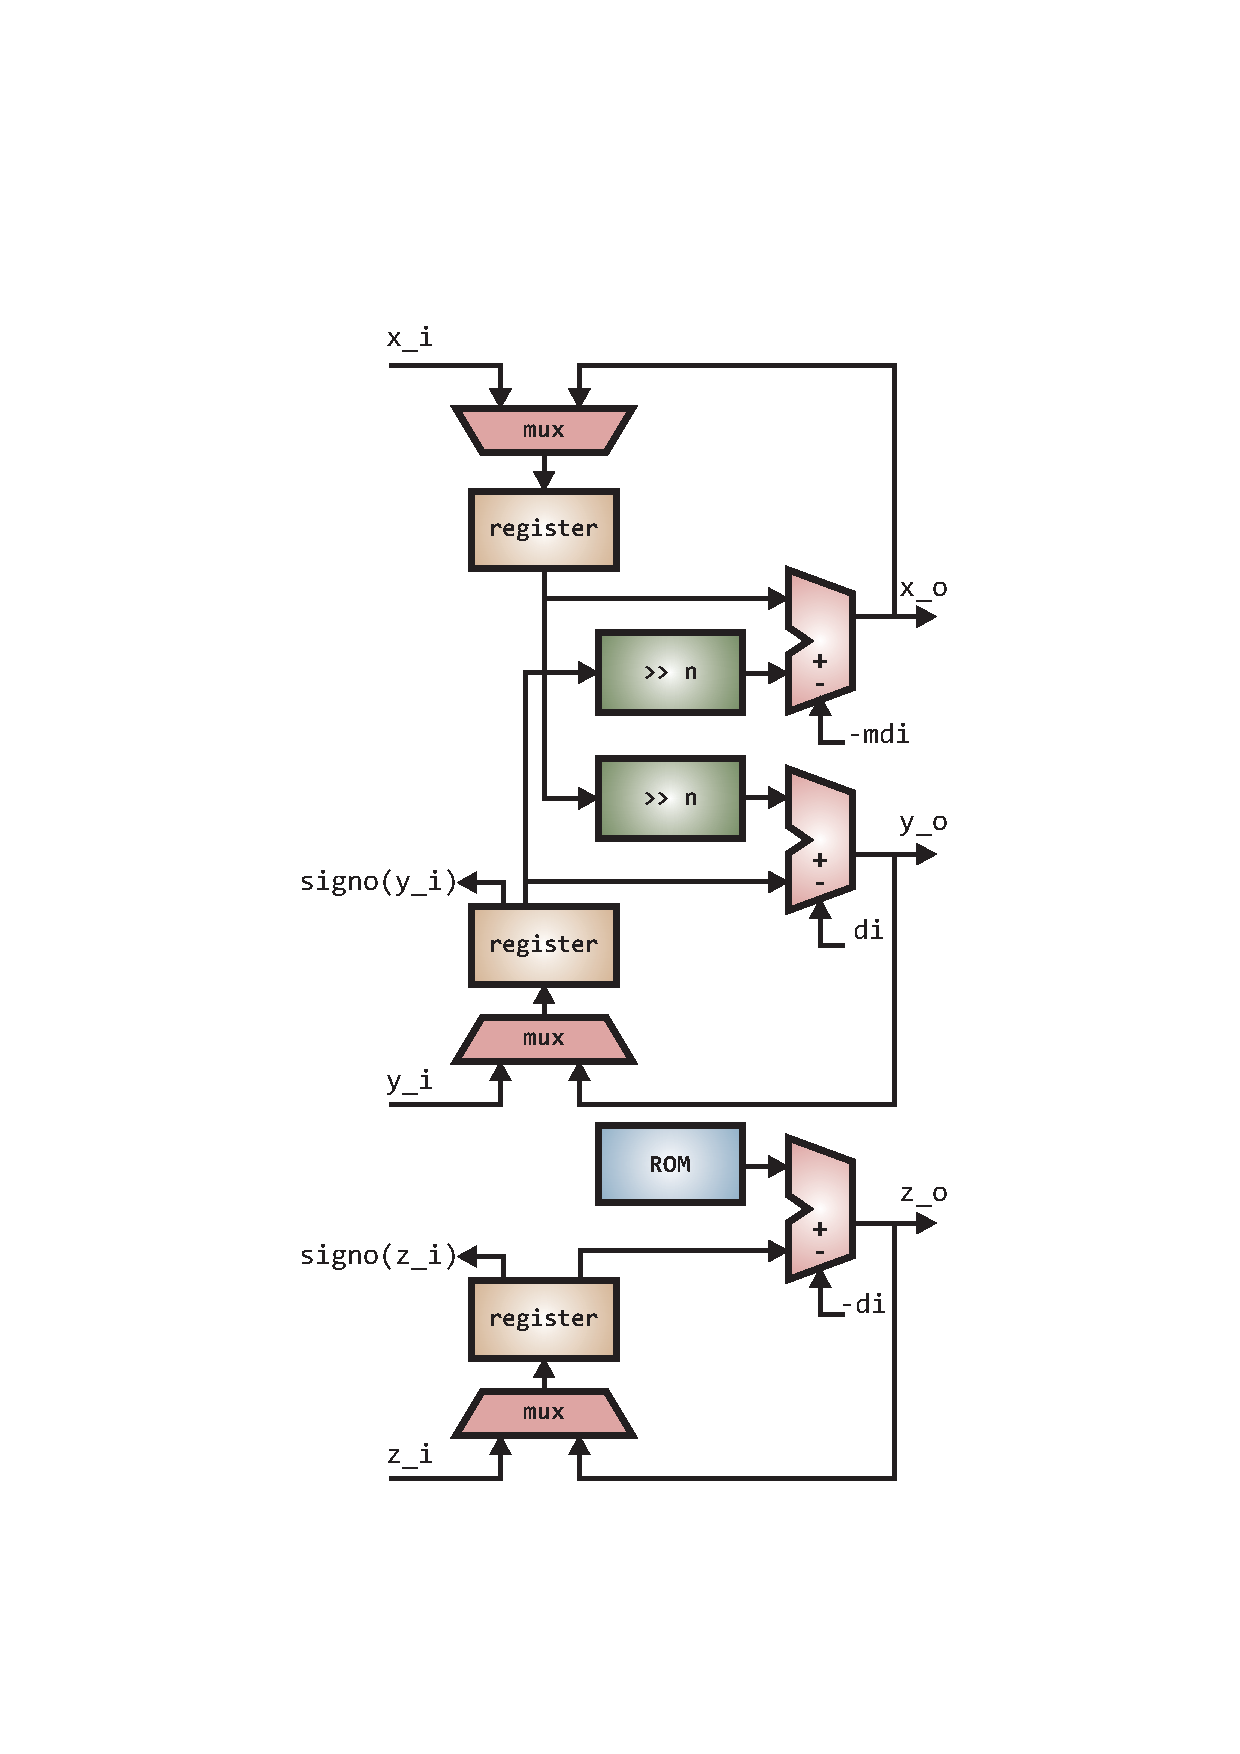
\includegraphics[width=7 cm]{./figures/C04-cordic_hardware}
 		\caption{Diagrama RTL de la implementación de CORDIC en hardware}
		\label{fig:cordic_hardware}
 	\end{center}
\end{figure}

\section{Post-multiplicador de salidas $x$ e $y$ de CORDIC}

El código \textbf{postmultiplier.v} describe el hardware desarrollado para hacer la atenuación requerida para compensar la ganancia de CORDIC. Es la última etapa del módulo de rotación ``\textit{rotator}'', y se aplica a las salidas de $x$ e $y$ de CORDIC. Según fue descripto en la sección \ref{subsec:El_algoritmo_CORDIC}, el hardware CORDIC introduce una ganancia $A_n$ al aplicar la rotación. Como en el hardware implementado es requerido que los vectores rotados no se vean escalados por la misma, se debe implementar una post-multiplicación que la atenúe.

Para implementar dicha multiplicación se hizo uso de la primitiva de producto del lenguaje Verilog, siendo la implementación definida al momento de la síntesis.

\section{Unidad de rotación completa}

El código \textbf{rotator.v} describe el hardware desarrollado para implementar un rotador el cual, utilizando los módulos de CORDIC, pre-procesamiento y post-multiplicación, sea capáz de manejar las operaciones BC e IC correctamente, sin importar el ángulo de los vectores de entrada (conformados por los valores de $R$ y $x$) y sin producir escalamientos. Para lograrlo, dicho hardware instancia un pre-procesador, un módulo CORDIC iterativo, dos post-multiplicadores (uno para $x$ y otro para $y$), y adicionalmente contiene el hardware de ajuste de ángulo requerido para los casos en que se utilice el modo vectorización y el vector de entrada tenga un ángulo mayor $\pi/2$ en módulo.

A continuación se expone un diagrama en bloques de la composición del rotador:

\begin{figure}[!h]
 	\begin{center}
 		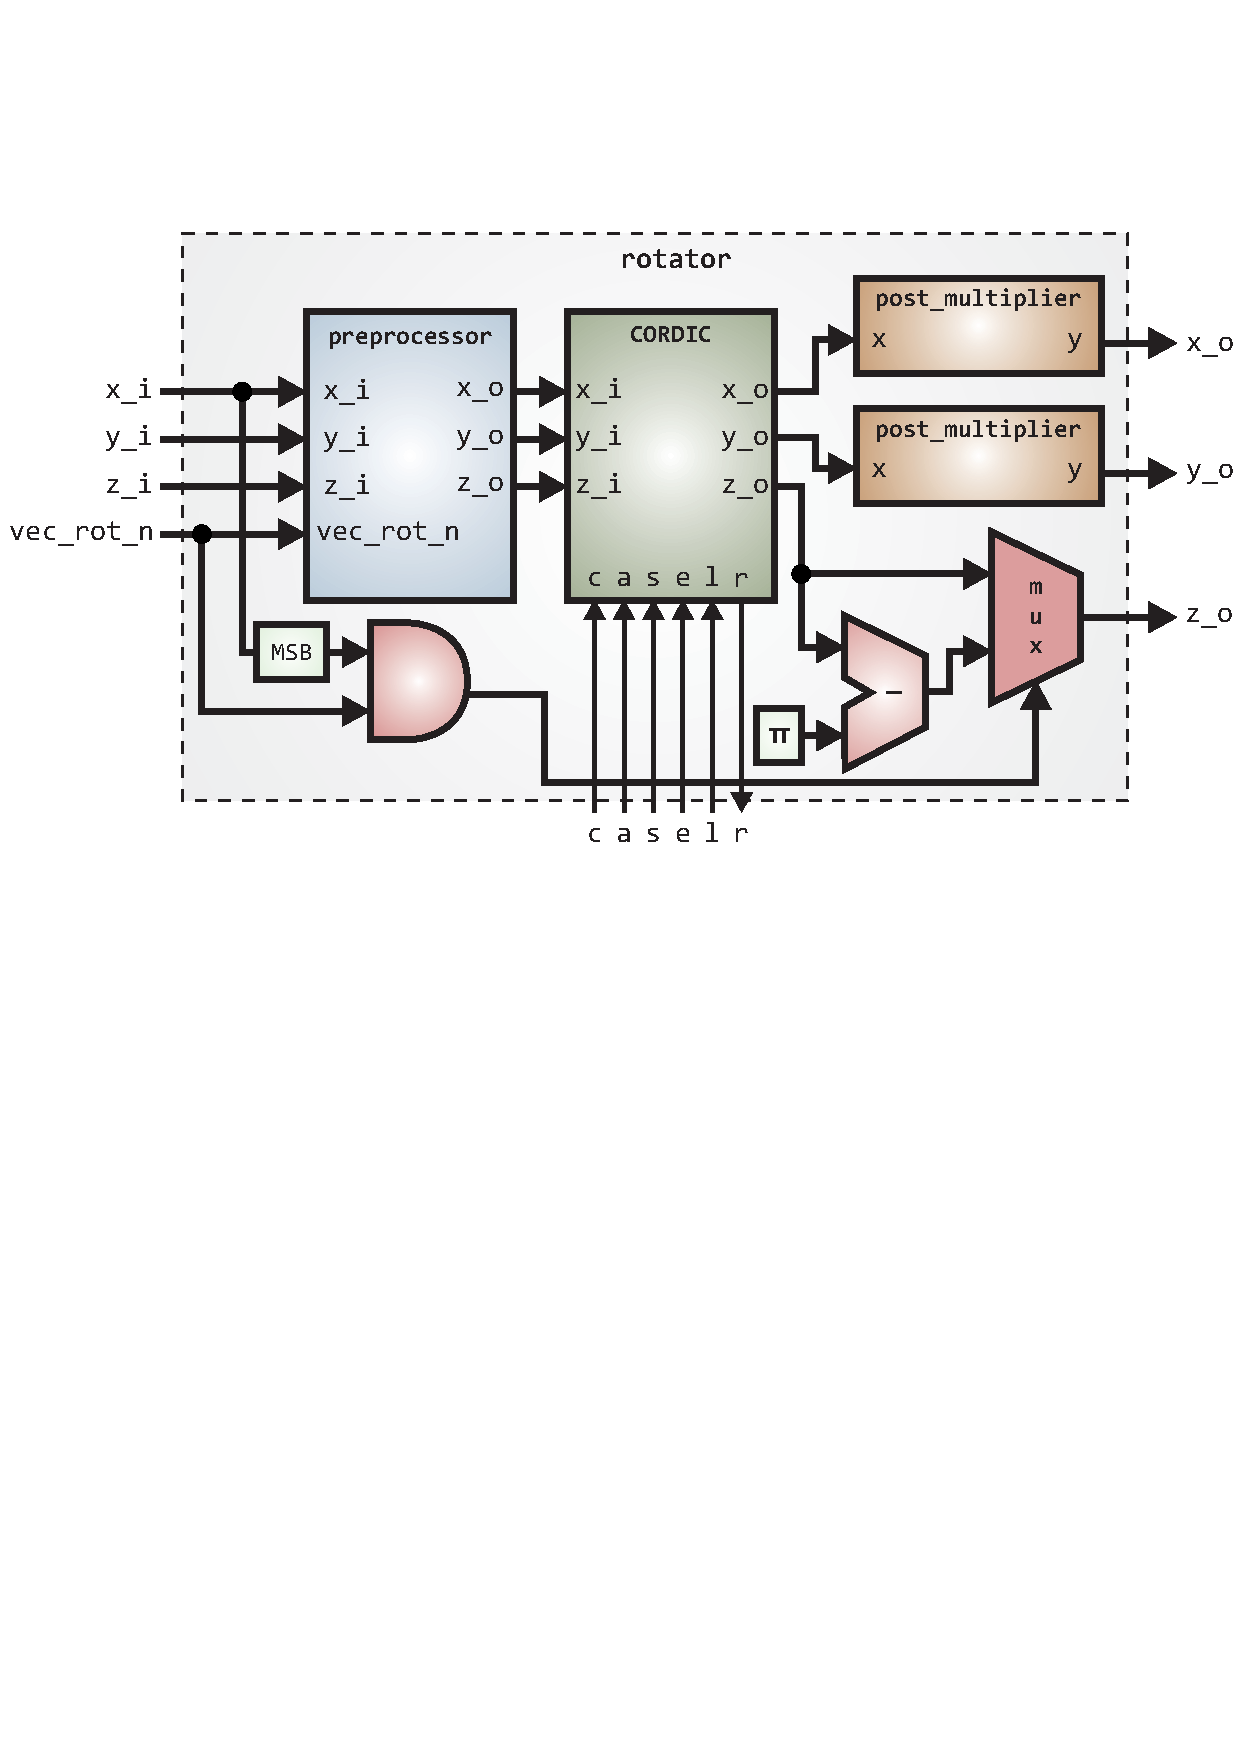
\includegraphics[width=15 cm]{./figures/C04-rotator_diagram}
 		\caption{Diagrama en Bloques del Módulo de Rotación}
		\label{rotator_diagram}
 	\end{center}
\end{figure}

\section{Procesador boundary cell}

El código \textbf{boundary\_cell.v} describe el hardware desarrollado para implementar las operaciones BC del procesador de descomposición QR. Las mismas fueron descriptas en la sección \ref{sec:descomposicion_qr} y se rigen por las ecuaciones \ref{eq:boundary_cell_1}, \ref{eq:boundary_cell_2} y \ref{eq:boundary_cell_3}. Para lograr la implementación de dichas ecuaciones, en el mismo se instancia un módulo rotador y se direccionan adecuadamente los valores de $R$ y $x$ de entrada, y los valores de $R_{new}$ y $angle$ de salida. El modo de operación del rotador se define de forma constante como modo vectorización.

\section{Procesador internal cell}

El código \textbf{internal\_cell.v} describe el hardware desarrollado para implementar las operaciones IC del procesador de descomposición QR. Las mismas fueron descriptas en la sección \ref{sec:descomposicion_qr} y se rigen por las ecuaciones \ref{eq:internal_cell_1} y \ref{eq:internal_cell_2}. Para lograr la implementación de dichas ecuaciones, en el mismo se instancia un módulo rotador y se direccionan adecuadamente los valores de $R$, $x$ y $angle$ de entrada, y los valores de $R_{new}$ y $x_{new}$ de salida. El modo de operación del rotador se define de forma constante como modo rotación.

\section{Procesador de descomposición QR}

El código \textbf{qr\_processor.v} es el \textit{top module} del proyecto y describe el hardware desarrollado para implementar el procesador de descomposición QR. A través de la definición de la unidad de registros, la lógica de control y la instanciación e interconexión de los módulos de celda que fueron descriptos, el mismo logra la implementación en hardware del algoritmo descripto.

La organización del código está distribuida como sigue:

\begin{enumerate}
	\item Definición del \textit{layout} del módulo, el cual incluye sus parámetros, entradas y salidas.
	\item Definición de los estados de control.
	\item Definición de registros e interconexiones.
	\item Instanciación de circuitos (\textit{boundary\_cell} e \textit{internal\_cell}).
	\item Definición de la arquitectura.
\end{enumerate}

\newpage

\subsection{Interfaz del módulo}

A continuación se describen las entradas y salidas del módulo:

\begin{itemize}
	\item[ ] \textbf{Entradas:}
	\item[•] \verb;clk;    : Entrada de \textit{clock} del sistema. El hardware opera por detección de flanco ascendente.
	\item[•] \verb;arst;   : \textit{Reset} asincrónico activo en alto.
	\item[•] \verb;srst;   : \textit{Reset} sincrónico  activo en alto.
	\item[•] \verb;enable; : \textit{Enable} sincrónico activo en alto.
	\item[•] \verb;start;  : \textit{Flag} para indicar que se está suministrando un nuevo vector de entrada, el cual dispara el cálculo para una nueva matriz R.
	\item[•] \verb;lambda_option; : Selector de factor de olvido.
	\item[•] \verb;x_in_1; : Primer elemento del vector de entrada.
	\item[•] \verb;x_in_2; : Segundo elemento del vector de entrada.
	\item[•] \verb;x_in_3; : Tercer elemento del vector de entrada.
	\item[•] \verb;x_in_4; : Cuarto elemento del vector de entrada.
	\item[•] \verb;x_in_5; : Quinto elemento del vector de entrada.
	\item[•] \verb;x_in_6; : Sexto elemento del vector de entrada.
	\item[•] \verb;x_in_7; : Séptimo elemento del vector de entrada.
\end{itemize}

\begin{itemize}   
	\item[ ] \textbf{Salidas:}
	\item[•] \verb;ready;      : Cuando se encuentra en estado alto, indica que el resultado se encuentra disponible. La matriz de salida va a ser enviada, de a una fila por ciclo de clock, en las salidas \verb;y_out; donde cada una de ellas representa cada columna.
	\item[•] \verb;y_out_1;    : Primera columna de la fila correspondiente de la matriz de salida.
	\item[•] \verb;y_out_2;    : Segunda columna de la fila correspondiente de la matriz de salida.
	\item[•] \verb;y_out_3;    : Tercera columna de la fila correspondiente de la matriz de salida.
	\item[•] \verb;y_out_4;    : Cuarta columna de la fila correspondiente de la matriz de salida.
	\item[•] \verb;y_out_5;    : Quinta columna de la fila correspondiente de la matriz de salida.
	\item[•] \verb;y_out_6;    : Sexta columna de la fila correspondiente de la matriz de salida.
	\item[•] \verb;y_out_7;    : Séptima columna de la fila correspondiente de la matriz de salida.
\end{itemize}

\subsection{Uso del procesador QR}

La implementación del procesador desarrollada es capáz de calcular la descomposición QR de una matriz de $7 \times 7$. La salida es la matriz $R$, la cual contiene la información requerida de la matriz de entrada. La matriz $Q$ forma una base ortogonal que al ser multiplicada por $R$ equivale a la matriz de entrada. 

Si bien es posible computar la matriz $Q$ haciendo uso de los ángulos de salida calculados en las \textit{boundary cells}, o agregando hardware de triangularización adicional, no se realiza dicha implementación dado que la misma no es requerida para la aplicación elegida, en la cual el objetivo es el cálculo del vector de pesos de un \textit{beamformer}.

En esta aplicación, las columnas de la matriz de entrada se generan por las últimas $7$ muestras de $6$ antenas (primeras $6$ columnas, vector $x$) y una secuencia de entrenamiento (última columna, elemento $y$).

Dado el carácter recursivo de la implementación, para suministrar la matriz de entrada es necesario hacerlo de a una fila por vez. Se comienza suministrando la primera fila, activando el \textit{flag} \verb;start;, y esperando a que la señal de ready se coloque en estado en alto antes de suministrar la próxima fila. Se presenta en la figura \ref{fig:hardware_use} un diagrama de tiempos al insertar una primera fila $A = [a_1\ a_2\ a_3\ a_4\ a_5\ a_6\ a_7]$. Dicho proceso se debería repetir con las 6 filas restantes de la matriz.

\begin{figure}[!h]
 	\begin{center}
 		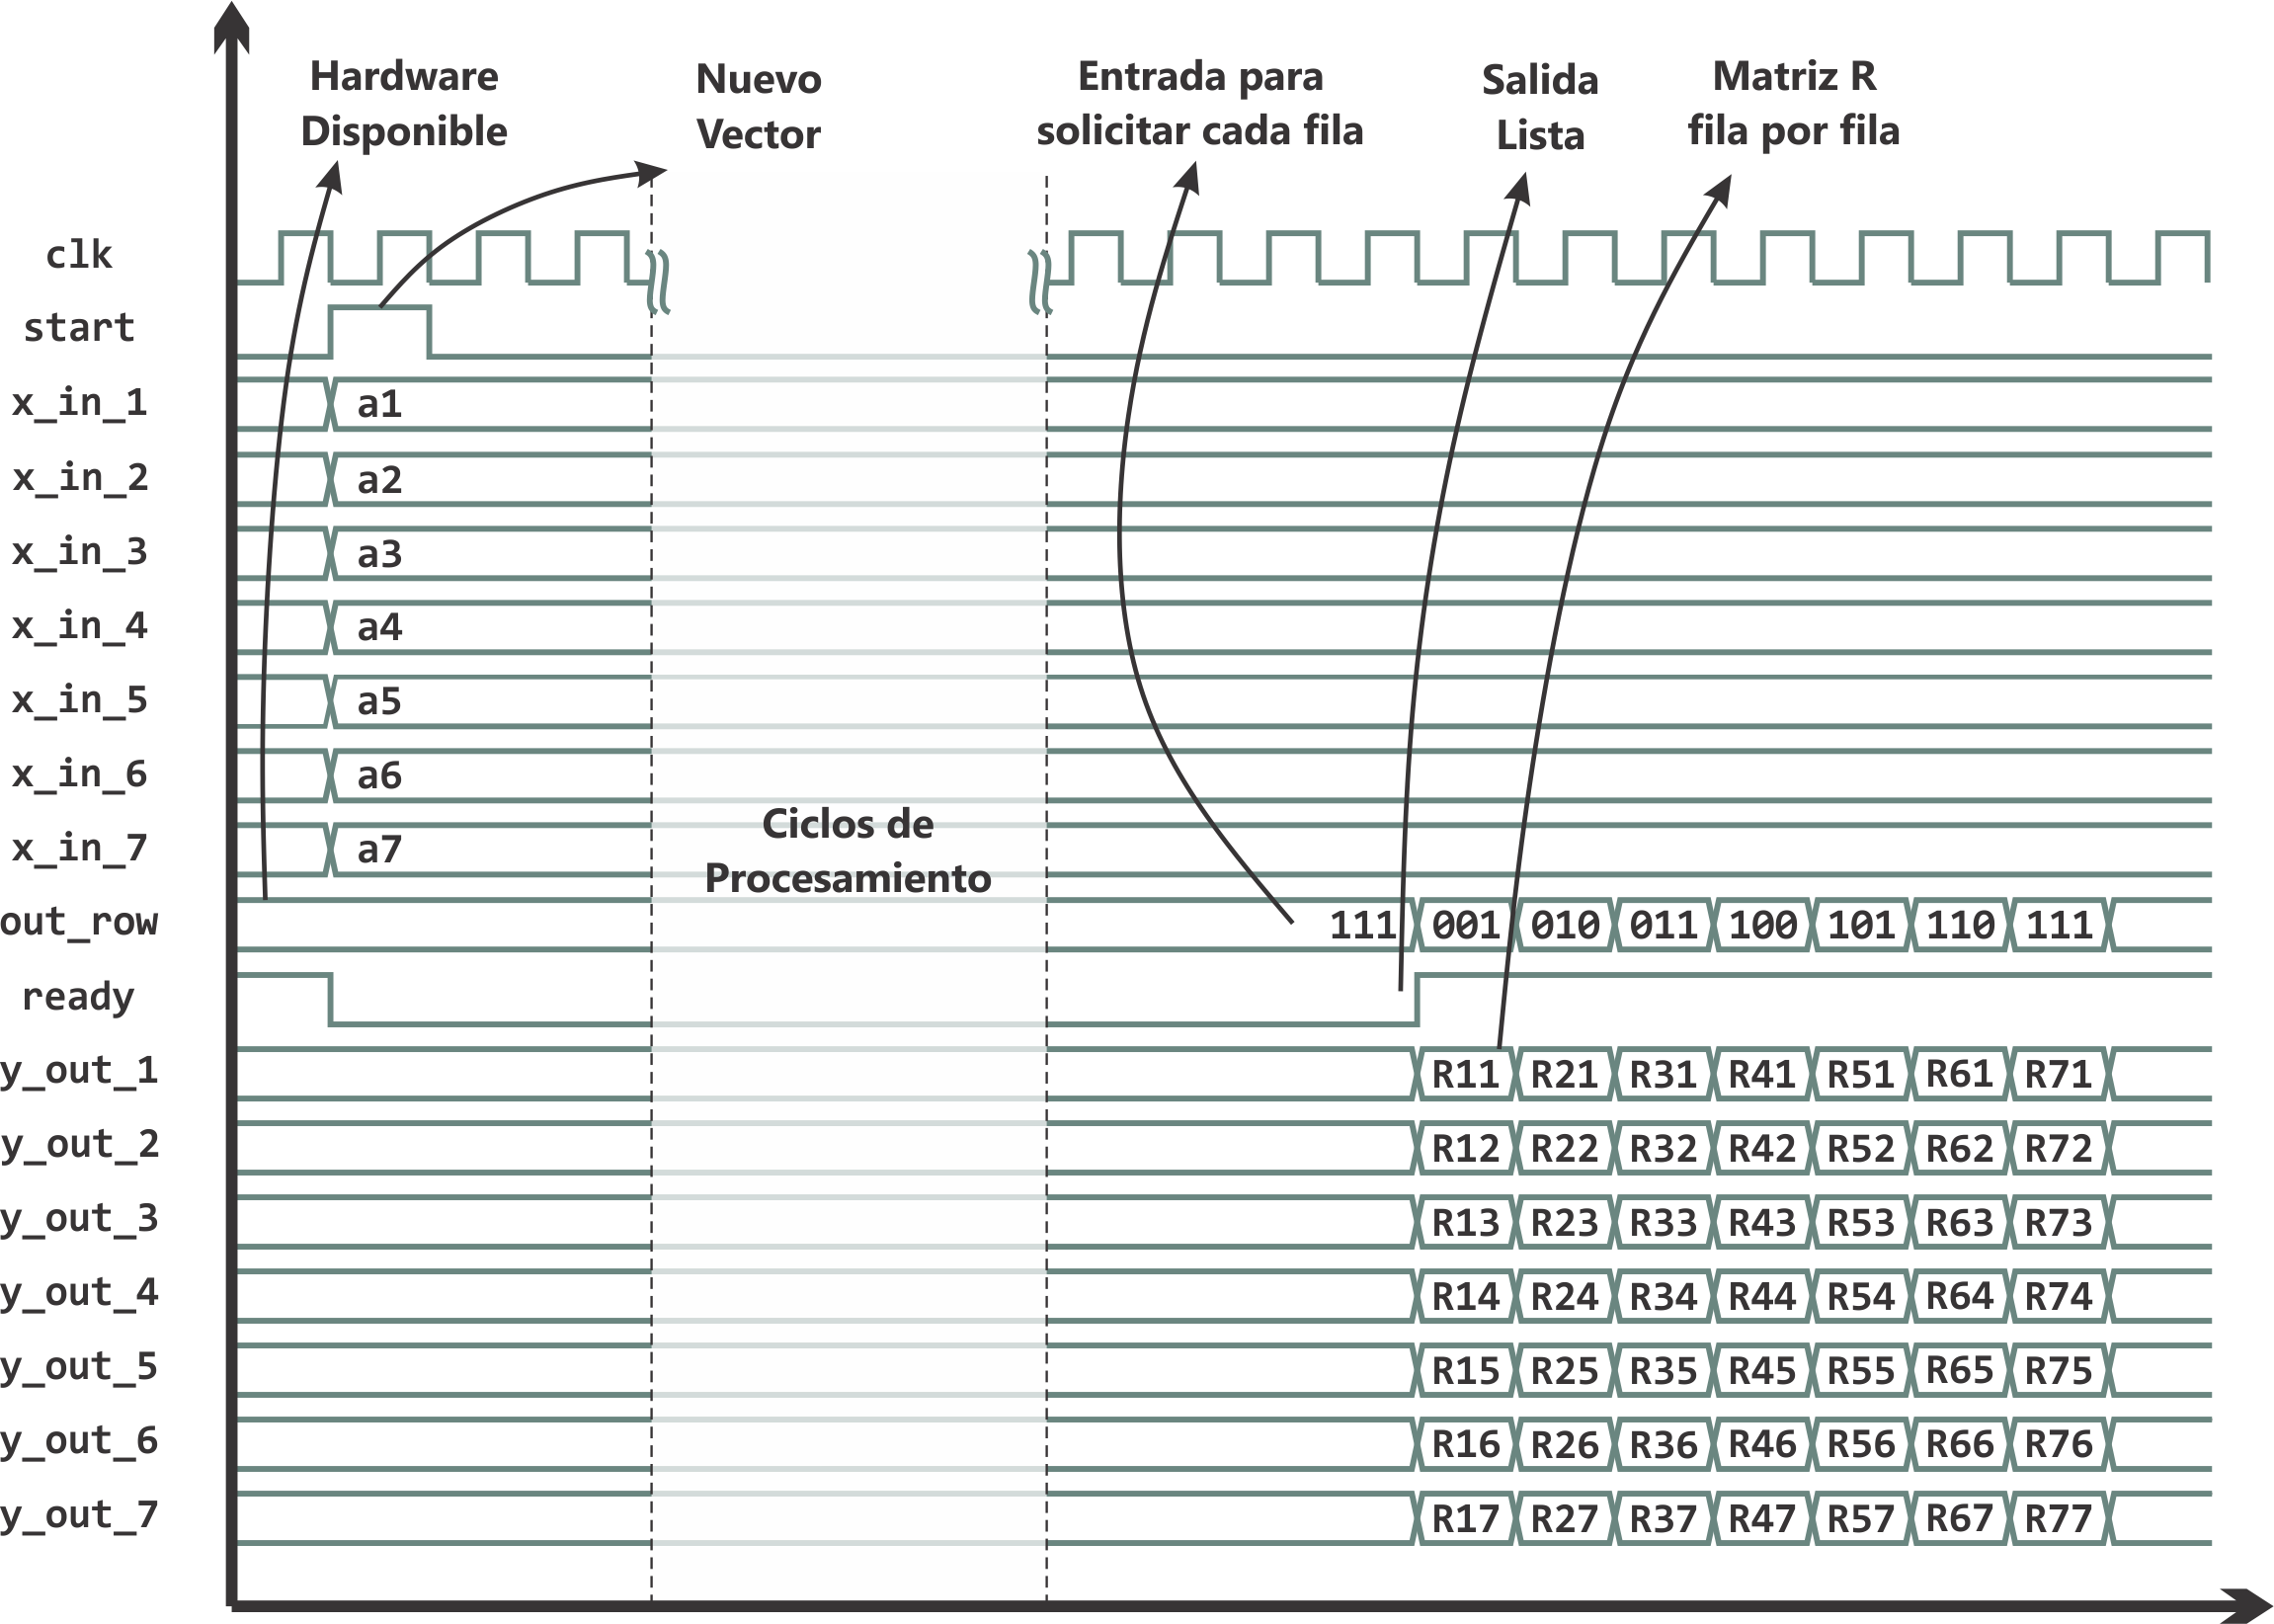
\includegraphics[width=11 cm]{./figures/C04-hardware_use}
 		\caption{Diagrama de Tiempos en el uso del Hardware}
		\label{fig:hardware_use}
 	\end{center}
\end{figure}

La composición de la matriz es siempre generada por un desplazamiento hacia abajo de las filas, en el cual se pierde la última fila, e ingresa en la primera el nuevo vector de entrada suministrado. Esta implementación recursiva se adapta al proceso de \textit{beamforming}, donde las filas que se mantienen representan las últimas 6 muestras. Este comportamiento se observa en la figura \ref{fig:hardware_cycles}. En la imagen se debe notar, por un lado el cambio en cada procesamiento, donde se observa el resultado anterior desplazado, y por el otro, la pérdida de la última fila en el Octavo Procesamiento.

\begin{figure}[!h]
 	\begin{center}
 		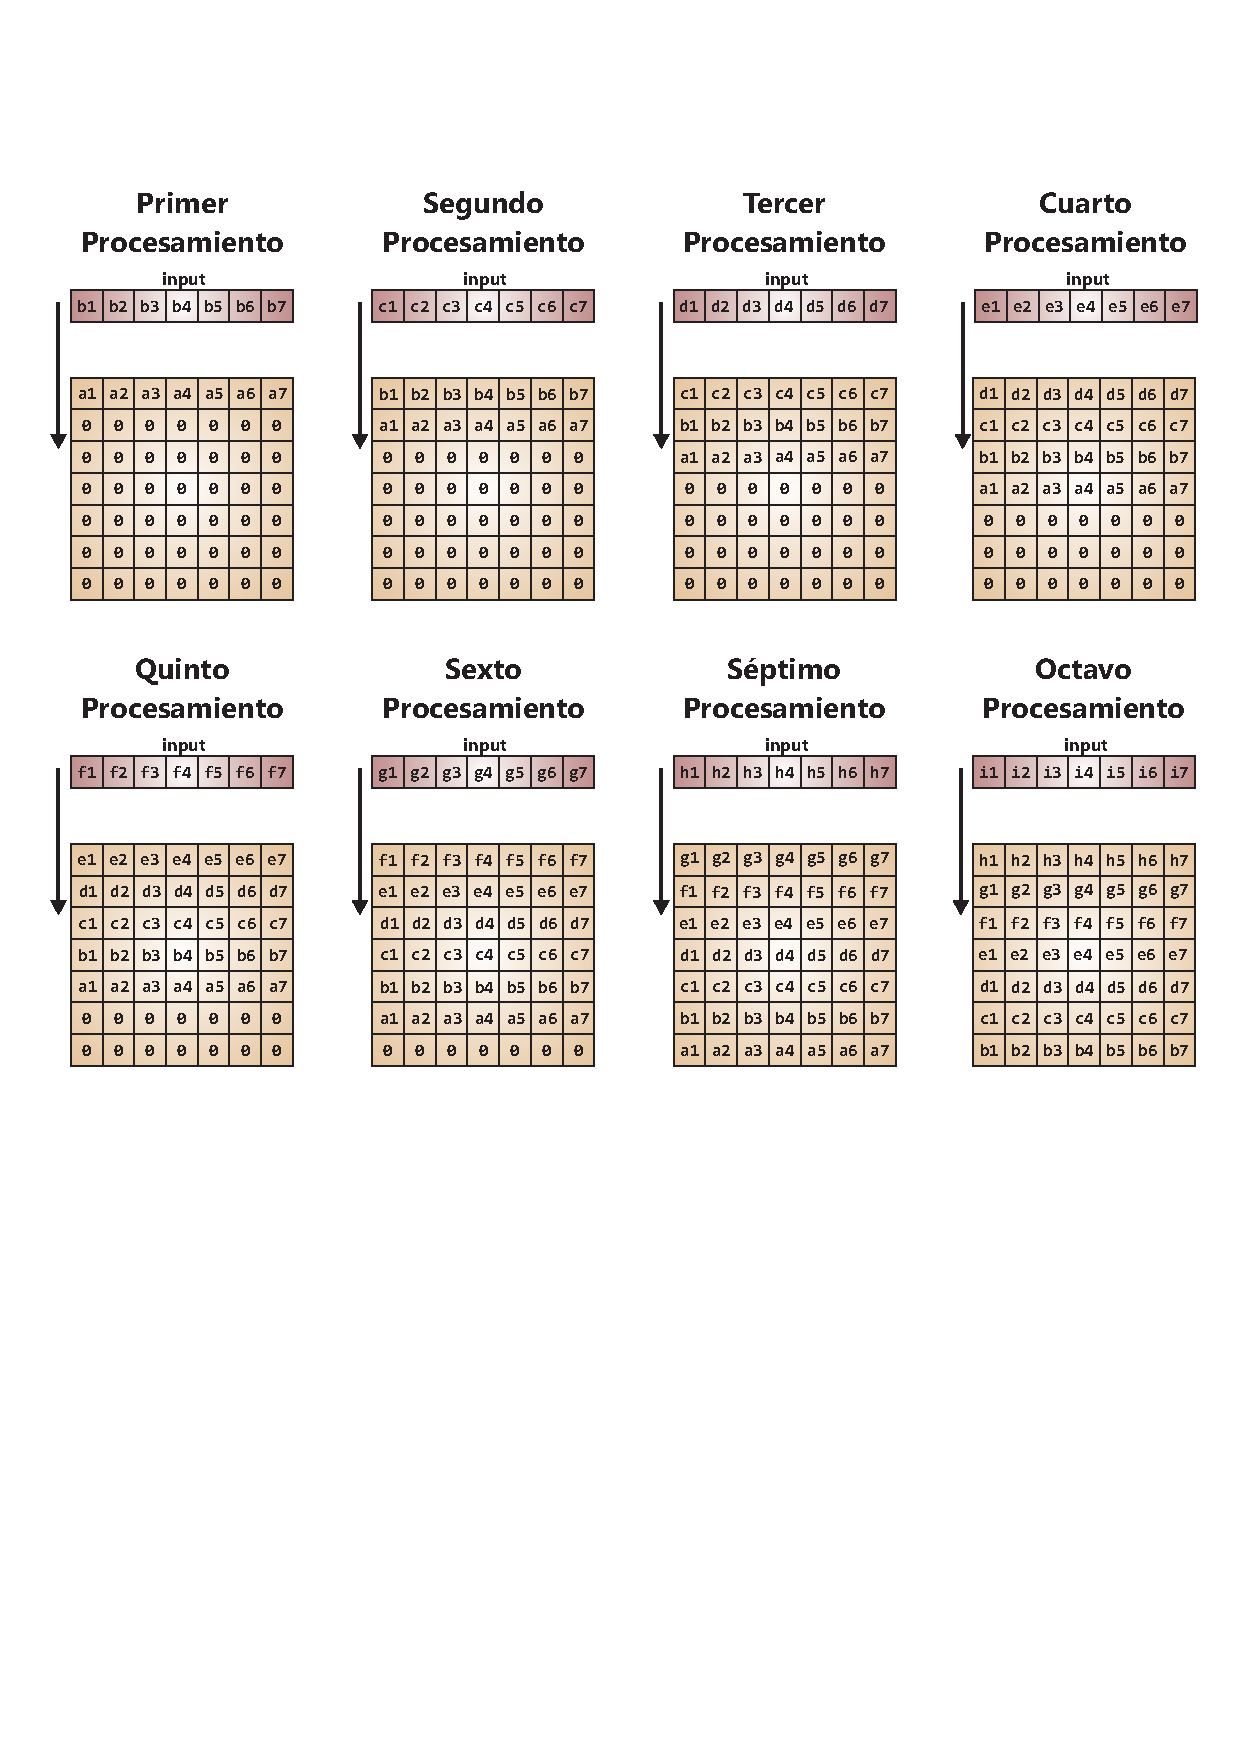
\includegraphics[width=13 cm]{./figures/C04-hardware_cycles}
 		\caption{Esquema de los primeros 8 ciclos de procesamiento}
		\label{fig:hardware_cycles}
 	\end{center}
\end{figure}

La matriz de entrada completa nunca es almacenada en los registros internos del procesador, dado que no es necesario contar con la misma. Si fuese un requerimiento, fácilmente se podría incorporar la misma en la unidad de registros desarrollada.

Si se deseara calcular una matriz completamente nueva, se debe repetir el proceso de suministrar cada fila esperando a que se active la señal de \textit{ready}.

\newpage

\subsection{Unidad de registros}

A continuación se hará una descripción detallada de la forma en la cual se almacenan y utilizan los elementos de una matriz en hardware. En la sección \ref{subsec:mapeo_de_walke}, se explicó que es necesario retener los valores de $R$ de una iteración, para la siguiente. En el mapeo de Walke, al reducir la arquitectura, se requiere que no sólo los valores de $R$ se almacenen, sino también los de $x$, y al ser varios pares $(x,R)$ asignados a un mismo procesador, esto es requerido para varios ciclos.

Esta implementación podría haber sido realizada dentro de las celdas, pero en lugar de hacerlo de esta forma, se optó por crear una unidad de registros, que tenga ciertas propiedades particulares para dar ventajas a la ejecución del algoritmo. Tanto la unidad de registros, como la forma en la cual se opera, es un diseño propio que presenta diversas ventajas para el mapeo, y fue ideado específicamente durante el desarrollo.

Como se vio en el diagrama en bloques, el esquema de almacenamiento de datos es el siguiente:

\begin{figure}[!h]
 	\begin{center}
 		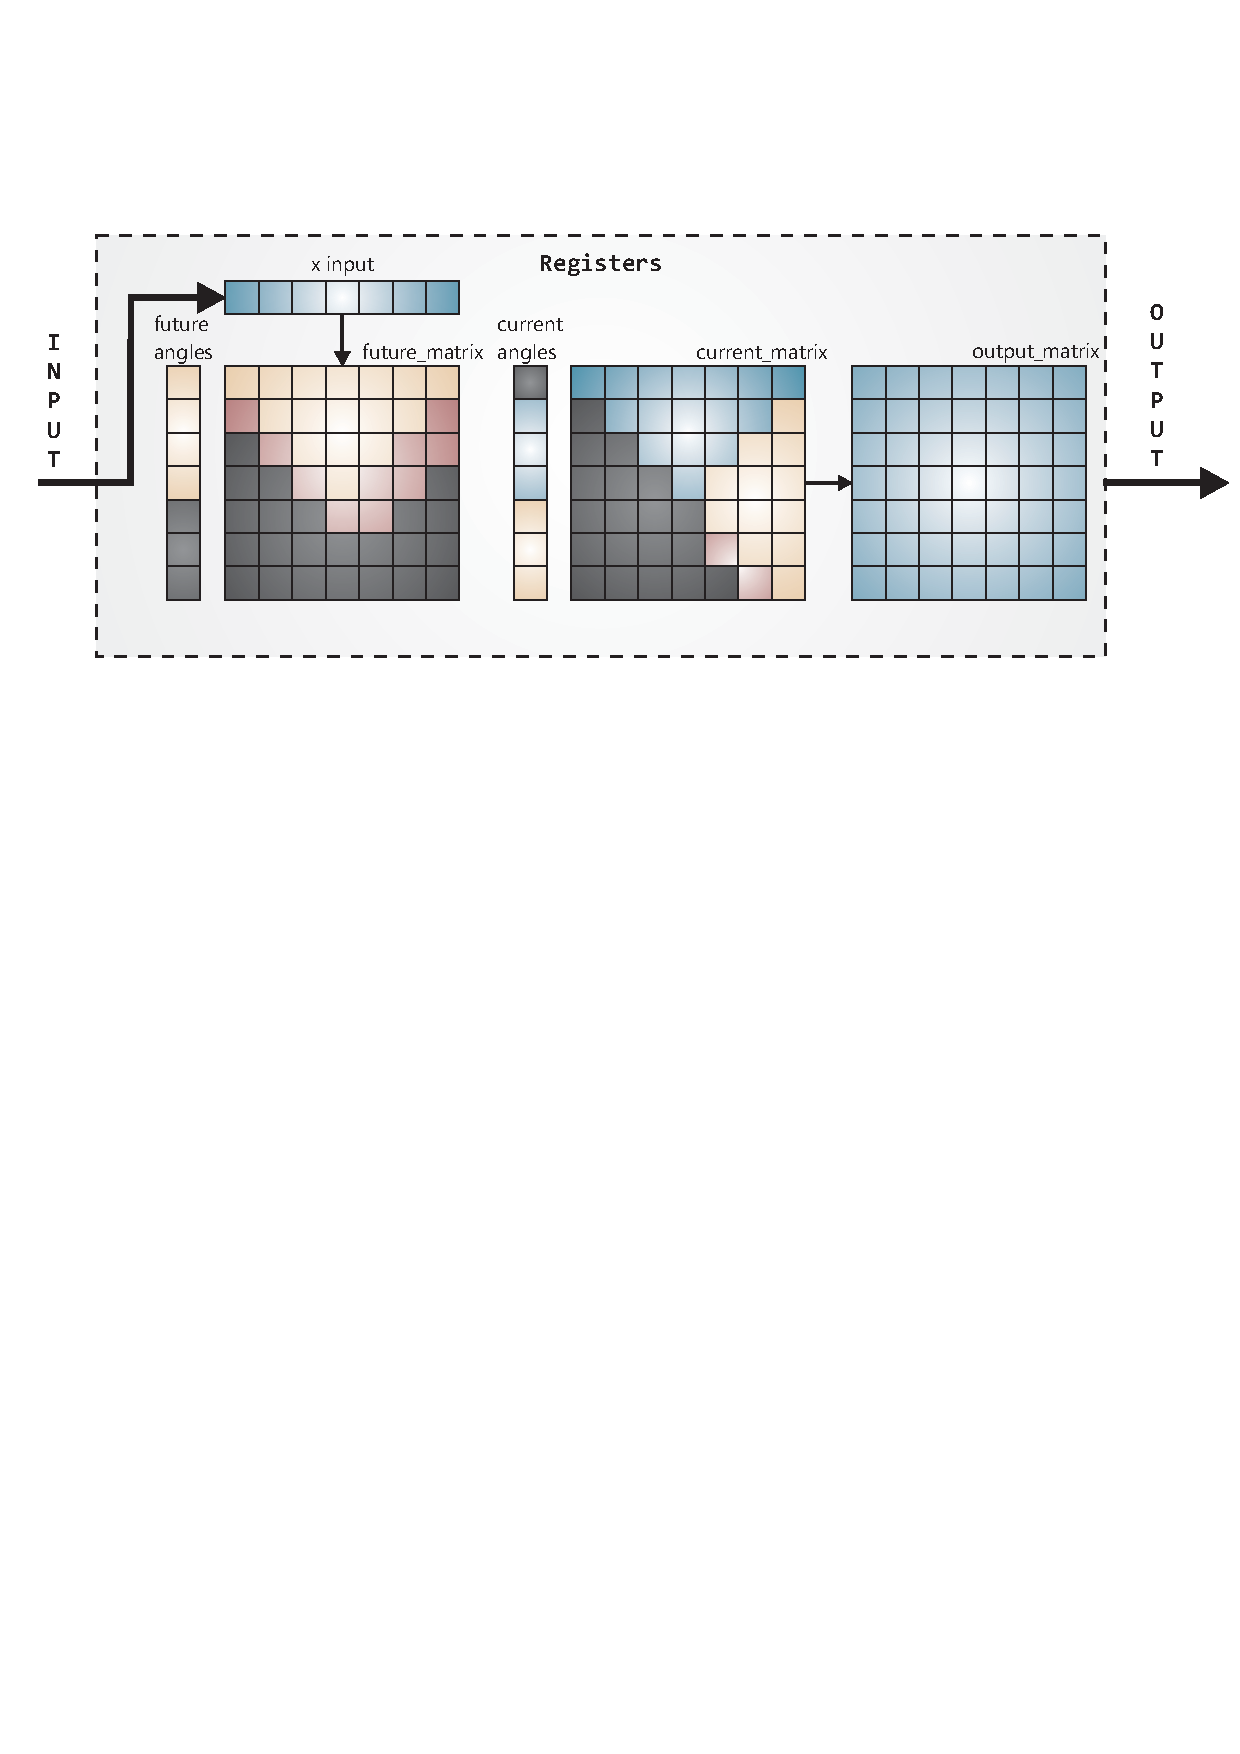
\includegraphics[width=15 cm]{./figures/C04-registers}
 		\caption{Esquema de registros utilizados}
		\label{fig:registers}
 	\end{center}
\end{figure}

Una de las características del mapeo de Walke, es que para lograr la máxima eficiencia de los procesadores, mientras algunos de ellos están procesando el ciclo actual, otros están procesando datos para el ciclo futuro. Por lo cual, en un determinado ciclo de procesamiento se deben almacenar los elementos calculados para dos entradas diferentes. Por este motivo existen las unidades de registros \verb;current_matrix; y \verb;future_matrix;, las cuales son de tamaño \verb;M x N x WORD_WIDTH;. Respectivamente, los ángulos calculados en las operaciones de \textit{boundary cell} son uno por fila, y son almacenados en los registros \verb;current_angles; y \verb;future_angles;.

Finalmente, el bloque de registros \verb;output_matrix; es utilizado para retener el resultado del cálculo de descomposición de una matriz durante toda la etapa de procesamiento, desde que se coloca en alto la señal de \textit{ready} al final de un ciclo, hasta que ocurre el mismo suceso en el siguiente.

Es importante destacar que la lógica de control y los pasos requeridos para la implementación del algoritmo serán descriptos con mayor detalle, y en este caso sólo se explican brevemente las características de los registros.

Se puede observar en el diagrama de la figura \ref{fig:registers} que los elementos de la matriz poseen diferentes colores. Cada uno de ellos representa una característica del registro. Las mismas se describen a continuación:

\begin{itemize}
	\item[•] \textbf{Color Azul}: El color azul representa un registro que se actualiza una única vez durante todo el procesamiento de una matriz. El primer caso es el del registro \verb;x_input;, donde se almacena el nuevo vector de entrada, el cual, concatenado con la matriz anterior, crea la nueva matriz. Luego se tiene un bloque de forma triangular en la parte superior de \verb;current_matrix;. En el mismo, se realiza una copia de los valores de \verb;future_matrix; para luego tenerlos disponibles en los estados de procesamiento. Esto es realizado en una de las etapas tempranas del algorimo. Este es el mismo caso que se da con la primera mitad de \verb;current_angles;. Finalmente, \verb;output_matrix; permanece constante durante todo el procesamiento con el último cálculo de matriz realizado, y se actualiza en el último estado del algoritmo.
	
	\item[•] \textbf{Color Dorado}: Representa un bloque de registros que forman parte del procesamiento del algoritmo, y cambia continuamente durante el mismo. En ellos, se almacenan cada una de las entradas y salidas modificadas por las \textit{boundary\_cells} e \textit{internal\_cells}. El primer caso se da en la matriz \verb;future_matrix;, donde se empieza a calcular una matriz que será finalizada en el próximo ciclo. Por ejemplo, en el ciclo 1 de procesamiento, se utilizan los registros de las posiciones $(1;1)$ y $(2;1)$ de esta unidad. Por otro lado, se tiene la matriz \verb;current_matrix;, donde se almacena el cálculo de la matriz actual, y se utilizan los valores previamente calculados en el sitio anterior. Para seguir con el ejemplo del ciclo 1, se utilizan los registros de las posiciones $(4;5), (5;5), (2;7), (3;7), (3;6), (4;6)$. Finalmente, se tienen los registros donde se leen y escriben los ángulos calculados.
	
	\item[•] \textbf{Color Rojo}: Además de ser registros con las mismas características que poseen los registros dorados, este color representa un registro utilizado para mantener un valor que es requerido en el próximo procesamiento, que sería perdido al realizar el desplazamiento hacia abajo.
	
	\item[•] \textbf{Color Negro}: Representa un registro que no es utilizado. Estos registros se encuentran presentes dado que en Verilog los mismos son creados definiendo los bloques en forma de arreglos bidimensionales. Se verá que, como posibles mejoras, se puede lograr unificar la matriz de salida con estos registros en conjunto con otros adicionales.
\end{itemize}

\subsection{Unidad de control}

A continuación se describirá la unidad codificada para el control del procesador de descomposición QR. La misma fue codificada como una máquina de estados finita. Dado que los estados son consecutivos, la síntesis resulta en un contador, pero la descripción como máquina de estados permite, además de una lectura y entendimiento del código más amigable, el escalamiento del mismo en el futuro. A continuación se describen cada uno de los estados:

\begin{itemize}
	\item[•] \textbf{wait\_vector}: Se trata del estado \textit{idle} del procesador en el que se encuentra a la espera de un nuevo vector, el cual es detectado a través de la señal \verb;start; en alto. El vector que es suministrado desde las entradas del procesador es almacenado en el bloque de registros \verb;future_matrix; en la fila 0. Esto representa una diferencia con el diagrama de registros visto, en el cual se observa un registro separado denominado \verb;x_input;. Se debe tener presente que la fila 0 \textbf{no} es una fila válida de matriz, dado que tanto filas como columnas comienzan desde el subíndice $1$. El registro 0, presente en todos los casos, es agregado como un auxiliar que en este caso es utilizado para almacenar una nueva entrada.
		
	\begin{figure}[h!]
	 	\begin{center}
	 		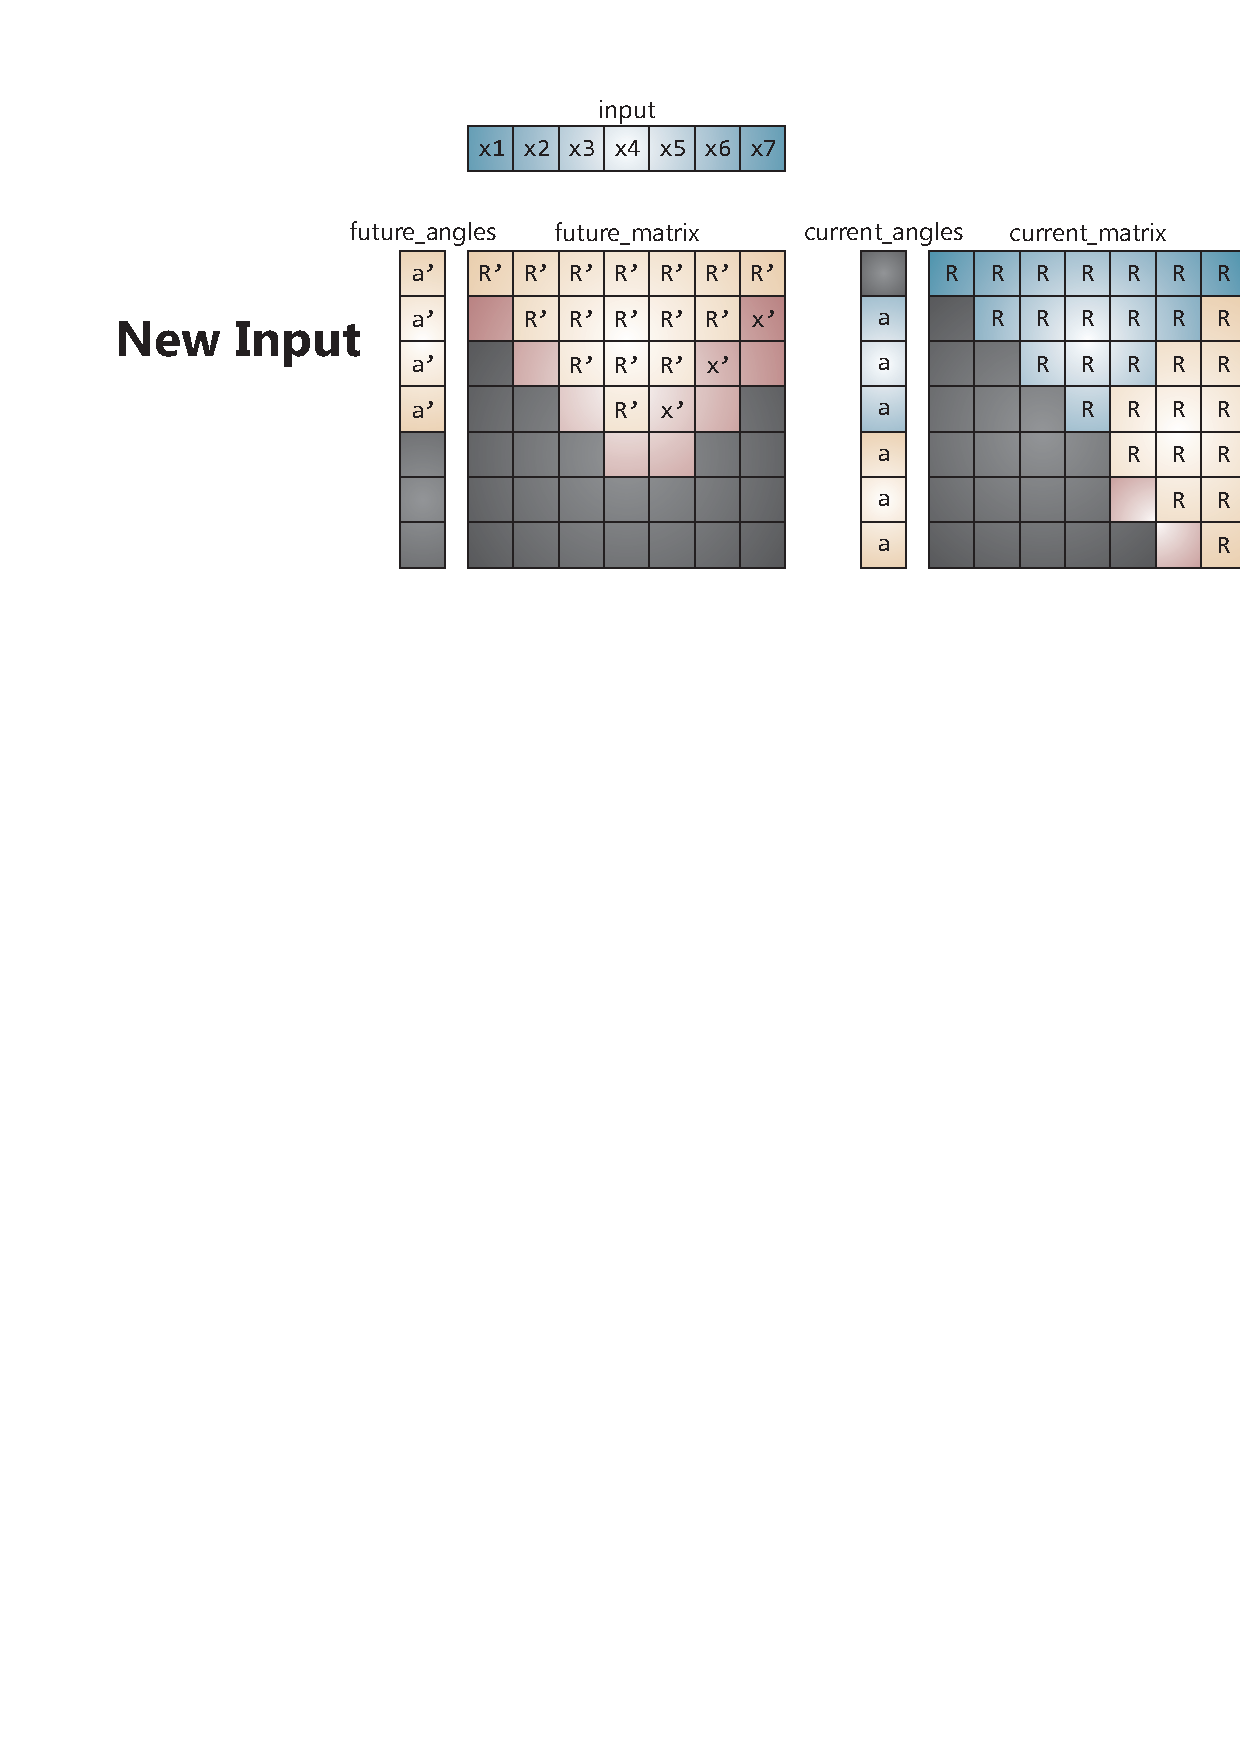
\includegraphics[width=12 cm]{./figures/C04-algorithm_new_input}
	 		\caption{Detección de nueva entrada y estado inicial}
			\label{fig:algorithm_new_input}
	 	\end{center}
	\end{figure}
	
	\item[•] \textbf{shift\_down}: En este estado, con excepción del bloque de registros de salida, se desplazan todos los registros hacia abajo. En \verb;future_matrix;, dado que en la posición $0$ se tiene el nuevo vector $x$, la nueva fila ingresa a la matriz en la fila $1$, se desplazan hacia abajo las demás, y se pierde la última. Los otros registros, con excepción de \verb;output_matrix;, donde no es necesario, también son desplazados hacia abajo para alinearse con el cambio originado por la nueva entrada.
	
	\begin{figure}[h!]
	 	\begin{center}
	 		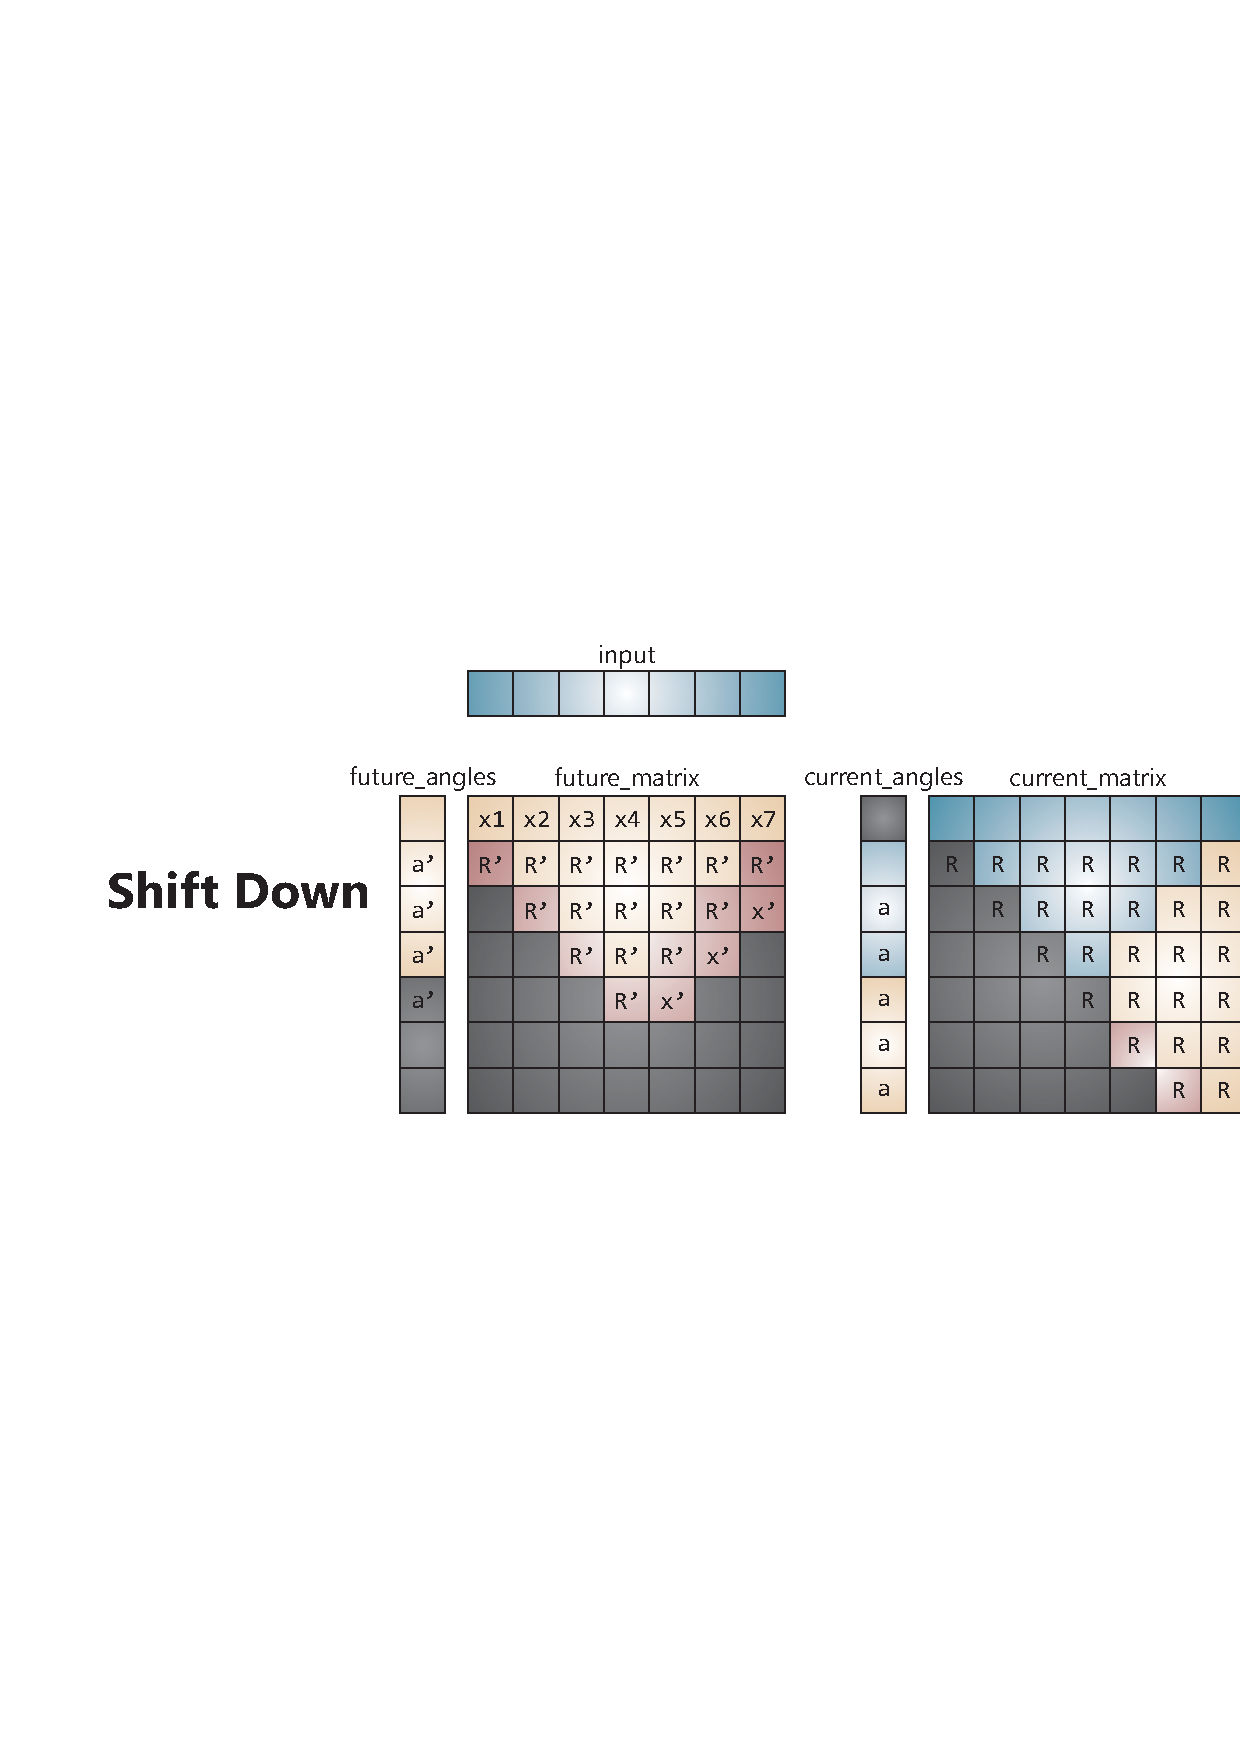
\includegraphics[width=12 cm]{./figures/C04-algorithm_shift_down}
	 		\caption{Resultado del desplazamiento hacia abajo}
			\label{fig:algorithm_shift_down}
	 	\end{center}
	\end{figure}

	\newpage
	
	\item[•] \textbf{copy\_matrix}: Una vez realizado el desplazamiento, se debe realizar una copia de los valores actuales en \verb;future_matrix; a la matriz \verb;current_matrix;. Dichos valores son aquellos que fueron calculados en el procesamiento anterior y conforman la primera mitad del cálculo actual. Se copian los valores de $R$ y de $x$. Adicionalmente, en este estado se comprueba si el vector recibido es el primer vector. En dicho caso, no es necesario hacer ningún procesamiento dado que para que el mismo sea válido es requerido que ingresen en los registros por lo menos dos vectores. Si la comprobación es acertada, se vuelve al estado \verb;wait_vector;.
	
	\begin{figure}[h!]
	 	\begin{center}
	 		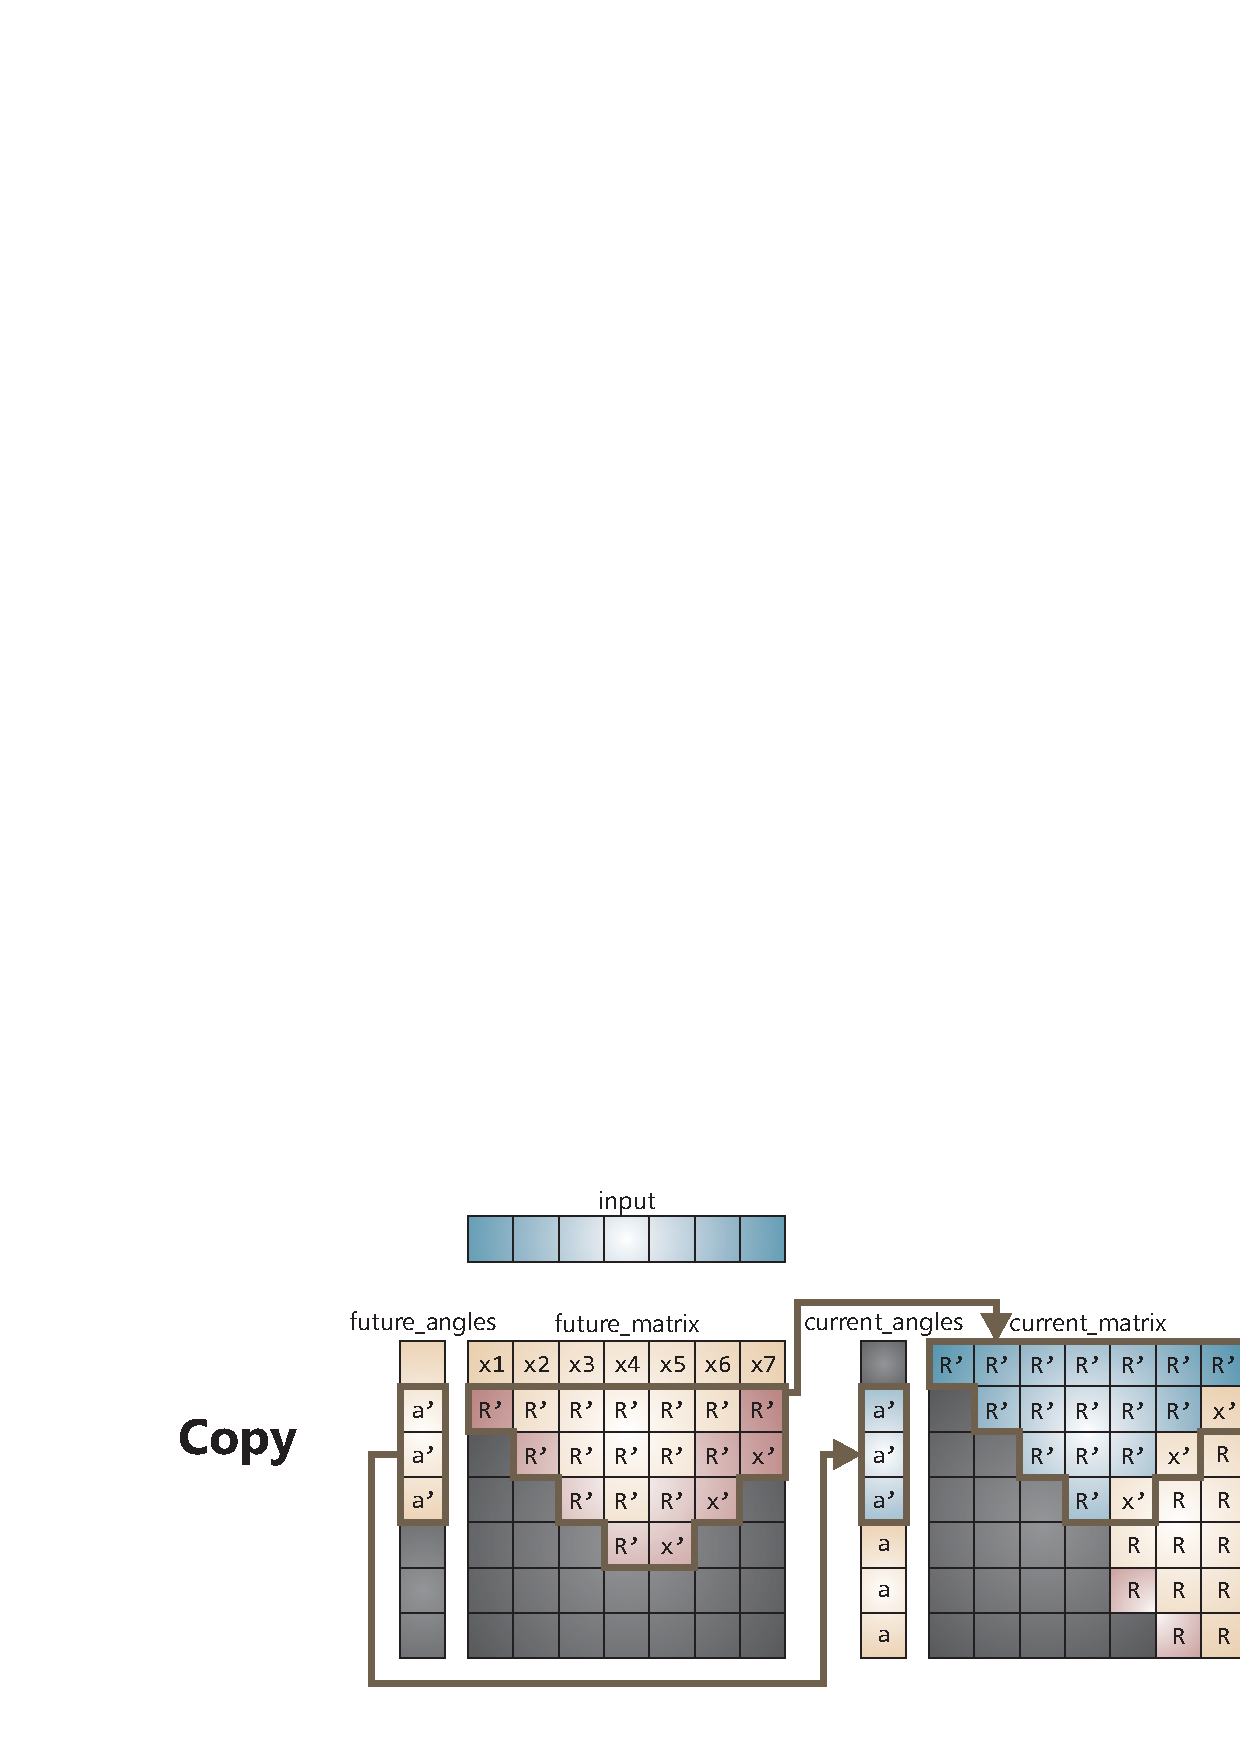
\includegraphics[width=12 cm]{./figures/C04-algorithm_copy}
	 		\caption{Resultado de la copia}
			\label{fig:algorithm_copy}
	 	\end{center}
	\end{figure}

	
	\item[•] \textbf{load\_cycleN} y \textbf{process\_cycleN}: Posterior a la copia, se tiene una serie de estados denominados \verb;load_cycle; y \verb;process_cycle; junto con un número, los cuales consisten en los $N$ estados de procesamiento de los valores $R$ y $x$ de la matriz. En los mismos, se redireccionan las entradas y salidas de las celdas BC e IC, y se controlan las señales de \verb;load; y \verb;ready; para que cada una de las celdas lleve a cabo la rotación correspondiente según las rotaciones de Givens.
	
	Básicamente, el estado \textit{load} consiste en colocar en estado alto la señal \verb;load; suministrando las entradas correspondientes al estado en proceso. Al pasar al siguiente estado, denominado \textit{process}, se pone en estado bajo la señal de \textit{load} y se espera a que todas las celdas coloquen en alto la señal de ready. Una vez detectado dicho suceso, las salidas de las celdas son almacenadas en los registros y el proceso se repite en la siguiente iteración.
	
	\item[•] \textbf{output\_results}: En este estado, se realiza una copia de la imagen actual del bloque de registros \verb;current_matrix; al bloque \verb;output_matrix;. Dado que la unidad \verb;current_matrix; es constantemente modificada durante los ciclos de procesamientos, es requerido copiarlos si se desea retenerlos. Existe un hardware adicional, activado por la señal \verb;send_output;, que lee los valores de la \verb;ouput_matrix; y los escribe en las señales de salida, uno por ciclo de \textit{clock} del procesador QR.
\end{itemize}

En el siguiente capítulo se describirán todos los resultados obtenidos en las simulaciones y síntesis del hardware implementado.

\section{Herramientas utilizadas}

A continuación se hace una breve reseña de las herramientas utilizadas para la implementación del procesador:

\subsubsection*{Sublime Text 2}
\begin{wrapfigure}{r}{0.22\textwidth}
	\vspace{-15pt}
	\begin{center}
		
\includegraphics[width=0.20\textwidth]{./figures/C04-logo_sublime}
	\end{center}
	\vspace{-15pt}
\end{wrapfigure}
Sublime Text fue el principal editor de texto utilizado para codificar en lenguaje Verilog. El mismo presenta una interfaz gráfica con diferentes características de gran utilidad.

\subsubsection*{Vim}
\begin{wrapfigure}{r}{0.22\textwidth}
	\vspace{-20pt}
	\begin{center}
		
\includegraphics[width=0.15\textwidth]{./figures/C04-logo_vim}
	\end{center}
	\vspace{-20pt}
\end{wrapfigure}
Vim es un editor de texto nativo en entornos de tipo UNIX y fue utilizado en algunos casos en conjunto con Sublime Text 2.

\subsubsection*{ModelSim}
\begin{wrapfigure}{r}{0.22\textwidth}
	\vspace{-15pt}
	\begin{center}
		
\includegraphics[width=0.20\textwidth]{./figures/C04-logo_modelsim}
	\end{center}
	\vspace{-15pt}
\end{wrapfigure}
ModelSim fue la herramienta utilizada para la simulación del hardware descripto en código fuente Verilog, con la cual se generaron los archivos de salida de tipo \textit{wave}.

\subsubsection*{gtkwave}
\begin{wrapfigure}{r}{0.22\textwidth}
	\vspace{-15pt}
	\begin{center}
		
\includegraphics[width=0.20\textwidth]{./figures/C04-logo_gtkwave}
	\end{center}
	\vspace{-15pt}
\end{wrapfigure}
Gtkwave fue la herramienta utilizada para visualizar los archivos de tipo \textit{wave} que fueron generados por la simulación realizada en ModelSim.

\subsubsection*{Xilinx ISE}
\begin{wrapfigure}{r}{0.22\textwidth}
	\vspace{-15pt}
	\begin{center}
		
\includegraphics[width=0.15\textwidth]{./figures/C04-logo_ise}
	\end{center}
	\vspace{-15pt}
\end{wrapfigure}
ISE Design Suite es la herramienta proporcionada por la compañía Xilinx para crear los archivos de síntesis ``.bit'' a partir de un hardware codificado en un lenguaje HDL. Dichos archivos .bit implementan el hardware en los dispositivos FPGA que Xilinx provee (Spartan y Virtex, entre otros). También fue utilizada para transferir los archivos ``.bit'' al kit de desarrollo FPGA.

\subsubsection*{Bitbucket}
\begin{wrapfigure}{r}{0.22\textwidth}
	\vspace{-15pt}
	\begin{center}
		
\includegraphics[width=0.20\textwidth]{./figures/C04-logo_bitbucket}
	\end{center}
	\vspace{-15pt}
\end{wrapfigure}
Para realizar el desarrollo se utilizó un repositorio hospedado en \href{http://www.bitbucket.org}{http://www.bitbucket.org}, el cual fue utilizado a través de la herramienta de versionado Mercurial. Dicho sistema aportó diversas ventajas, entre las cuales principalmente se encuentran el mantener un registro de todas las modificaciones realizadas entre cada una de las versiones y el poder trabajar en la nube. En caso de algún comportamiento no deseado al hacer un cambio de versión, el mismo podía ser identificado en el registro proporcionado por la herramienta. El poder trabajar en la nube, facilitó el hecho de poder hacer aportes en el desarrollo desde distintos equipos, ya sea por estar en un equipo de la facultad, del hogar o del trabajo.